%!TEX TS-program = latexmk
%
% Copyright 2026 Martin Scheidt (ISC license)
% Permission to use, copy, modify, and/or distribute this file for any purpose with or without fee is hereby granted, provided that the above copyright notice and this permission notice appear in all copies.

\documentclass[border=3pt,convert={density=300,outext=.png}]{standalone}

\usepackage{tikz}
\usetikzlibrary{calc,shapes.geometric}
\newcommand{\diamonded}[1]{\tikz[baseline=(n.base)]{\node[draw,diamond,inner sep=0.5pt,thin,font=\tiny] (n) {#1};}}

\begin{document}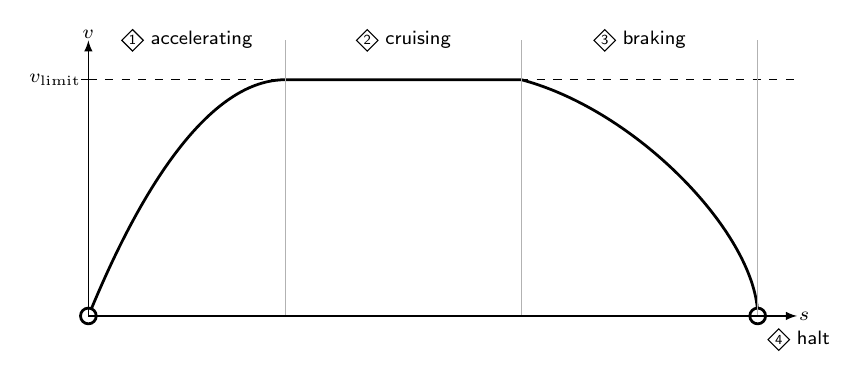
\begin{tikzpicture}[font=\sffamily]
  \tikzset{every node/.style={inner sep=0.5pt},font = {\scriptsize\sffamily}}
  \tikzstyle{grid}=[thin,black!30]

  \def\h{3.5}
  \def\s{3}
  \def\Xend{9}

  \coordinate (A) at (0,0);

  % speed limit
  \draw[line width=0.5pt,dashed] (0,\s) -- ++(\Xend,0);

  % dynamic speed profile: accelerate → cruise → brake → halt
  \draw[line width=1pt]
    (A) parabola[bend at end] (2.5,\s) coordinate (B) --
    ++(3,0) coordinate (C) .. controls ++(1.5,-0.4) and (8.5,1) .. (8.5,0) coordinate (E);
  \draw[line width=1pt,fill=white] (A) circle (0.1cm);
  \draw[line width=1pt,fill=white] (E) circle (0.1cm);

  % grid
  \draw[grid] let \p1 = (B) in (\x1,0) -- ++(0,\h);
  \draw[grid] let \p1 = (C) in (\x1,0) -- ++(0,\h);
  \draw[grid] let \p1 = (E) in (\x1,0) -- ++(0,\h);

  % labels
  \path let \p1 = (A),\p2 = (B) in (\x1,\h) -- (\x2,\h) node[pos=.5] {\diamonded{1} accelerating};
  \path let \p1 = (B),\p2 = (C) in (\x1,\h) -- (\x2,\h) node[pos=.5] {\diamonded{2} cruising};
  \path let \p1 = (C),\p2 = (E) in (\x1,\h) -- (\x2,\h) node[pos=.5] {\diamonded{3} braking};
  \node[align=left,below=0.3cm,right=0.1cm] at (E) {\diamonded{4} halt};

  % axis
  \draw[->,>=latex]    (A)       -- ++(\Xend, 0) node[right] {$s$};
  \draw[->,>=latex]    (A)       -- ++( 0   ,\h) node[above] {$v$};
  \draw[shorten <=3pt] (-0.2,\s) -- ++( 0.2 , 0) node[left=0.2em] {$v_\mathrm{limit}$};

\end{tikzpicture}\end{document}
